\documentclass[a4paper]{article}

\usepackage{indentfirst}
\usepackage[english]{babel}
\usepackage[utf8]{inputenc}
\usepackage{amsmath}
\usepackage{graphicx}
\usepackage[colorinlistoftodos]{todonotes}
\usepackage[useregional]{datetime2}
\usepackage{fancyhdr}
\usepackage{titlesec}
\usepackage{listings} 
\usepackage{hyperref}
\hypersetup{
    colorlinks=true,
    linkcolor=midnightblue,
    filecolor=magenta,      
    urlcolor=midnightblue,
}
\usepackage{caption}
\usepackage{titling}
\usepackage{upquote}

\usepackage{color}

 \usepackage{wrapfig}

\setcounter{secnumdepth}{4}

\setlength{\droptitle}{-4em}

\setlength{\intextsep}{6pt plus 2pt minus 2pt}

%Define colors as shown below to use in text.
\definecolor{midnightblue}{RGB}{20, 86, 128}
\definecolor{Red}{RGB}{255, 0, 0}
\definecolor{Green}{RGB}{0, 255, 0}
\definecolor{Blue}{RGB}{0, 0, 255}
\definecolor{codegreen}{rgb}{0,0.6,0}
\definecolor{codegray}{rgb}{0.5,0.5,0.5}
\definecolor{codepurple}{rgb}{0.58,0,0.82}
\definecolor{backcolour}{rgb}{0.95,0.95,0.92}

% code listing style
\lstset{language=Python}
\lstdefinestyle{mystyle}{
    backgroundcolor=\color{backcolour},   
    commentstyle=\color{codegreen},
    keywordstyle=\color{magenta},
    numberstyle=\tiny\color{codegray},
    stringstyle=\color{codepurple},
    basicstyle=\ttfamily\footnotesize,
    breakatwhitespace=false,         
    breaklines=true,                 
    captionpos=b,                    
    keepspaces=true,                 
    numbers=left,                    
    numbersep=5pt,                  
    showspaces=false,                
    showstringspaces=false,
    showtabs=false,                  
    tabsize=2
}
\renewcommand{\lstlistingname}{Code snippet}
 
\lstset{style=mystyle}


%Project Title
\newcommand{\projectTitle}{Data Visualization}
%Homework Number
\newcommand{\assignmentNumber}{2}

%Submission date goes here.
%Format: #Day of Month #Hour:#Minute AM/PM
\newcommand{\projectDate}{10th of May 11:59 PM}

%Contact to reach.
\newcommand{\contactName}{Hasan Can Aslan}
\newcommand{\contactMail}{haslan16@ku.edu.tr}

%Define colors as shown below to use in text.
\definecolor{Red}{RGB}{255, 0, 0}
\definecolor{Green}{RGB}{0, 255, 0}
\definecolor{Blue}{RGB}{0, 0, 255}

\author{Hasan Can Aslan}

\title{\projectTitle}

\date{Submission Date: \projectDate}

\begin{document}

\maketitle

\lstset{language=Python}
\pagestyle{fancy}
\fancyhf{}
\chead{\projectTitle}
\rhead{Assignment \#\assignmentNumber}
\lhead{KOLT Python}
\lfoot{\nouppercase{\leftmark}}
\rfoot{Page \thepage}
\thispagestyle{fancy}
\renewcommand{\headrulewidth}{0.4pt}
\renewcommand{\footrulewidth}{0.4pt}


\section{Introduction}

Each day, individuals across the globe collect terabytes of digital data for different purposes. Although the data vary in nature, we can think of data in their raw form as resources that lead us to new understandings. However, raw data could be noisy.

Data visualization is the process of mapping, graphing, plotting, and charting data to discover relationships and patterns. We will be creating data visualizations using \texttt{matplotlib} and \texttt{pandas} throughout this project. Your assignment consists of two parts: Ahmet's Lemons and Ceren's Garden Center. References and warm up exercises about related packages are provided before each part.


%Do not change this section.
\subsection{Submission}
We will use \emph{\href{https://okpy.org}{OK}} platform for assignment submissions. We already registered you, you should be able to see our class when you sign in using your Koç University mail address. Please contact us immediately if you have any issues. You should submit two files named \texttt\texttt{cerens\_garden\_center.py} and {ahmets\_lemons.py}.

%Do not change this section.
\subsection{Academic Honesty}
Koç University's \emph{\href{https://vpaa.ku.edu.tr/sites/vpaa.ku.edu.tr/files/Misc_Documents/Statement_on_Academic_Honesty.pdf}{Statement on Academic Honesty}} holds for all the homework given in this course. Failing to comply with the statement will be penalized accordingly. If you are unsure whether your action violates the code of conduct, please consult with your instructor.

%TODO: Write the aim of the project
\subsection{Aim of the Project}
In your homework assignments, the \textbf{functionality} and \textbf{style} of your programs are \textbf{both important.}  A program that “works” is not necessarily a good program. A good program is \textbf{comprehensible, readable and well structured.} Therefore you’re expected to decompose the main problem into \textbf{simpler subtasks} and \textbf{implement helper functions} for these subtasks. You’re also expected to write comments if needed, be careful about \textbf{indentation}, and use \textbf{descriptive names} for helper functions. Even if your program functions well according to the project requirements, you can still improve your code style and how you decompose the task. The goal of this project is to teach you how to see the meaning of a dataset and convey that information to others using Python.

%Do not change this section.
\subsection{Further Questions}
For further questions \textbf{about the project} you may contact \textbf{\contactName} at \href{mailto:\contactMail}{\mbox{[\contactMail]}}. Note that it may take up to 24 hours before you receive a response so please ask your questions \textbf{before} it is too late. No questions will be answered when there is \textbf{less than two days} left for the submission.

\section{Tasks}

\subsection{Pandas Reference}
This part consists of several functions and usages of \texttt{pandas}. Before proceeding to your assignment please read this part carefully. You \textbf{don't need to submit} any file for this part but we strongly recommend trying it on your own. Your next task will be built on these functions.

\subsubsection{Installing Pandas}
To use \texttt{pandas}, you need to install it from the PyPI. You can install it by writing your terminal following line: \\
\newline
\texttt{python -m pip install -U pandas} \\
\textbf{For Mac users:}\\
\texttt{python3 -m pip install -U pandas}

\subsubsection{Pandas}
\texttt{pandas} is an open-source library that is used to analyze data in Python. It takes in data, like a CSV or SQL database, and creates an object with rows and columns called a data frame. \texttt{pandas} are typically imported with the alias \texttt{pd}.

\begin{lstlisting}
import pandas as pd
\end{lstlisting}{}

\subsubsection{Pandas DataFrame Creation}
The fundamental \texttt{pandas} object is called a DataFrame. It is a 2-dimensional size-mutable, potentially heterogeneous, tabular data structure.

A DataFrame can be created in multiple ways. It can be created by passing in a dictionary or a list of lists to the \texttt{pd.DataFrame()} method, or by reading data from a CSV file.

\begin{lstlisting}
# Ways of creating a Pandas DataFrame
# Passing in a dictionary:
data = {'name':['Anthony', 'Maria'], 'age':[30, 28]}
df = pd.DataFrame(data)

# Passing in a list of lists:
data = [['Tom', 20], ['Jack', 30], ['Meera', 25]]
df = pd.DataFrame(data, columns = ['Name', 'Age'])

# Reading data from a csv file:
df = pd.read_csv('students.csv')
\end{lstlisting}{}

\subsubsection{Selecting Pandas DataFrame Rows Using Logical Operators}
In \texttt{pandas}, specific rows can be selected if they satisfy certain conditions using Python’s logical operators. The result is a DataFrame that is a subset of the original DataFrame.

Multiple logical conditions can be combined with OR (using \texttt{|}) and AND (using \texttt{\&}), and each condition must be enclosed in parentheses.

\begin{lstlisting}
# Selecting rows where age is over 20
df[df.age > 20]

# Selecting rows where name is not John
df[df.name != "John"]

# Selecting rows where age is less than 10
# OR greater than 70
df[(df.age < 10) | (df.age > 70)]
\end{lstlisting}{}

\subsubsection{Pandas apply() Function}
The \texttt{pandas} \texttt{apply()} function can be used to apply a function on every value in a column or row of a DataFrame, and transform that column or row to the resulting values.

By default, it will apply a function to all values of a column. To perform it on a row instead, you can specify the argument \texttt{axis=1} in the \texttt{apply()} function call.

\begin{lstlisting}
# This function doubles the input value
def double(x):
  return 2*x

# Apply this function to double every value in a specified column
df.column1 = df.column1.apply(double)

# Lambda functions can also be supplied to `apply()`
df.column2 = df.column2.apply(lambda x : 3*x)

# Applying to a row requires it to be called on the entire DataFrame
df['newColumn'] = df.apply(lambda row: 
  row['column1'] * 1.5 + row['column2'],
  axis=1)
\end{lstlisting}{}

\subsubsection{Pandas DataFrames Adding Columns}
\texttt{pandas} DataFrames allow for the addition of columns after the DataFrame has already been created, by using the format \texttt{df[\textquotesingle newColumn\textquotesingle]} and setting it equal to the new column’s value.

\begin{lstlisting}
# Specifying each value in the new column:
df['newColumn'] = [1, 2, 3, 4]

# Setting each row in the new column to the same value:
df['newColumn'] = 1

# Creating a new column by doing a 
# calculation on an existing column:
df['newColumn'] = df['oldColumn'] * 5
\end{lstlisting}{}

\subsection{Ceren's Garden Center}
Now you’re the data analyst for a chain of gardening stores called Ceren's Garden Center. As Ceren's business growing, getting harder to keep track of inventory. Help them analyze their inventory! Starter code-named \texttt{cerens\_garden\_center.py} for this part is provided. \textbf{You need to submit your answers for this part.}

\subsubsection{Answer Customer Emails}

\begin{itemize}
\item 
Data for all of the locations of Ceren's Garden Center is in the file \texttt{inventory.csv}. Load the data into a DataFrame called \texttt{inventory}.

\item
Inspect the first 10 rows of \texttt{inventory}.

\textbf{Hint:} You can slice dataframe like strings. For example, \texttt{df[:5]} or \texttt{df.head(5)} will return first 5 rows.

\item
The first 10 rows represent data from your Istanbul location. Select these rows and save them to \texttt{istanbul}.

\item
A customer just emailed you asking what products are sold at your Istanbul location. Select the column \texttt{product\_description} from \texttt{istanbul} and save it to the variable \texttt{product\_request}. 

\textbf{Hint:} You can select a column by writing its name in square brackets like \texttt{df[\textquotesingle product\_description\textquotesingle]}

\item
Another customer emails to ask what types of seeds are sold at the Bursa location.

Select all rows where \texttt{location} is equal to Bursa and\texttt{ product\_type} is equal to \texttt{seeds} and save them to the variable \texttt{seed\_request}. 

\textbf{Hint:} You can look at section 2.3.4 for examples about filtering.
\end{itemize}{}

\subsubsection{Inventory}

\begin{itemize}
\item 
Add a column to \texttt{inventory} called \texttt{in\_stock} which is \texttt{True} if \texttt{quantity} is greater than 0 and \texttt{False} if \texttt{quantity} equals 0. 

\textbf{Hint:} You can use the code in part 2.3.5 as an example with following changes: paste lambda below in \texttt{inventory.apply()}, and set its axis to \texttt{axis=1} to apply for each row.
\begin{lstlisting}
lambda row: row['quantity'] > 0
\end{lstlisting}{}

\item
Ceren's Garden Center wants to know how valuable their current inventory is.

Create a column called \texttt{total\_value} that is equal to \texttt{price} multiplied by \texttt{quantity}.

\textbf{Hint:} You can use the code in part 2.3.5 and task above as an example apply following lambda and set its axis to \texttt{axis=1} to apply for each row.
\begin{lstlisting}
lambda row: row['price'] * row['quantity']
\end{lstlisting}{}

\item
The Marketing department wants a complete description of each product for their catalog.

The following lambda function combines \texttt{product\_type} and \texttt{product\_description} into a single string:

\begin{lstlisting}
combine_lambda = lambda row: '{} - {}'.format(row.product_type, row.product_description)
\end{lstlisting}{}

Paste this function into \texttt{cerens\_garden\_center.py}.

\item
Using \texttt{combine\_lambda}, create a new column in inventory called \texttt{full\_description} that has the complete description of each product.

\textbf{Hint:} You just need to write \texttt{combine\_lambda} directly in the \texttt{inventory.apply()} and set its axis to \texttt{axis=1} to apply for each row.
\end{itemize}{}

\subsection{Matplotlib Reference}
This part consists of several functions of \texttt{matplotlib}. You can find a matplotlib cheat sheet at the \textbf{Resources} part at the end of the handout. You \textbf{don't need to submit} any file for this part, but we strongly recommend trying it on your own. Your next task will be built on these functions.

\subsubsection{Installing Packages}
To use \texttt{matplotlib}, you need to install it from PyPI (Python Package Index) using \texttt{pip} (Package installer for Python). \texttt{pip} comes pre-installed with modern distributions of Python. You can install \texttt{matplotlib} by writing your terminal following line: \\
\texttt{python -m pip install -U matplotlib} \\
\textbf{For Mac users:}\\
\texttt{python3 -m pip install -U matplotlib}

\subsubsection{Subplots in Matplotlib}
In Python, the \texttt{matplotlib}’s \texttt{pyplot.subplot()} the function can be used to create a figure with a grid of subplots. This function accepts the number of rows, number of columns, and the current index as arguments.

\begin{lstlisting}[caption={}]
import matplotlib.pyplot as plt
# Datasets
x = [1, 2, 3, 4]
y = [1, 2, 3, 4]

# First Subplot
plt.subplot(1, 2, 1)
plt.plot(x, y, color='green')
plt.title('First Subplot')

# Second Subplot
plt.subplot(1, 2, 2)
plt.plot(x, y, color='blue')
plt.title('Second Subplot')

# Display both subplots
plt.show()
\end{lstlisting}

\subsubsection{Figures in Matplotlib}
In \texttt{matplotlib} package, a figure is a container that holds plots. It can hold a single plot or multiple plots. When a figure holds multiple separate plots, those are called subplots.

\subsubsection{Setting Linestyle and Color in Matplotlib}
In \texttt{matplotlib} package, the \texttt{pyplot.plot()} function can accept parameters to set the color(\texttt{color}), linestyle(\texttt{linestyle}) and marker(\texttt{marker}) for line graph. Color values can be HTML color names or HEX codes. Line styles can be dashed(\texttt{\textquotesingle --\textquotesingle}) or dotted(\texttt{\textquotesingle ..\textquotesingle}). Markers can be circles(\texttt{\textquotesingle o\textquotesingle}), squares(\texttt{\textquotesingle s\textquotesingle}), stars(\texttt{\textquotesingle *\textquotesingle}), or other shapes.

\begin{lstlisting}[caption={}]
pyplot.plot(days, money_spent, color='green', linestyle='--')
pyplot.plot(days, money_spent_2, color='#AAAAAA',  marker='o')
\end{lstlisting}


\subsubsection{Pyplot Functions}
The \texttt{matplotlib} package contains the pyplot module, which provides users with an interface for graphing data. Pyplot contains over 100 functions, from acorr to yticks. You must import the module, and we recommend using \texttt{plt} to refer this module for your convenience.

\begin{lstlisting}
from matplotlib import pyplot as plt
\end{lstlisting}{}

Here are some of the most common pyplot functions: \\

\begin{table}[htb]
\begin{tabular}{lll}
\textbf{Function} &  & \textbf{Description}                     \\
\texttt{plot}              &  & plots y versus x as lines and/or markers \\
\texttt{show}              &  & displays a figure                        \\
\texttt{axis}              &  & sets some axis properties                \\
\texttt{xlabel}            &  & sets the label for the x-axis            \\
\texttt{ylabel}            &  & sets the label for the y-axis            \\
\texttt{title}             &  & sets a title for the axes                \\
\texttt{subplot}           &  & adds a subplot to the current figure     \\
\texttt{subplots\_adjust}  &  & tunes the subplot layout                 \\
\texttt{legend}            &  & places a legend on the axes              \\
\texttt{figure}            &  & creates a new figure                     \\
\texttt{savefig}           &  & saves the current figure                
\end{tabular}
\end{table}

\subsubsection{X-ticks and Y-ticks in Matplotlib}
In Python’s \texttt{matplotlib}, the x-tick and y-tick marks of the plot can be changed using functions \texttt{ax.set\_xticks()} and \texttt{ax.set\_yticks()}. These functions accepts an array of values representing tick mark positions.

\begin{lstlisting}
import matplotlib.pyplot as plt

ax = plt.subplot()
plt.plot([0, 1, 2, 3, 4], [0, 1, 4, 9, 16])
plt.plot([0, 1, 2, 3, 4], [0, 1, 8, 27, 64])
ax.set_xticks([1, 2, 4])
\end{lstlisting}{}

\subsection{Ahmet's Lemons}
In this part of the assignment, you will be acting as a data analyst for Ahmet who wants to start online retailing for his lemon business called Ahmet Lemons. People all over the country can use this product to get the freshest, best-quality lemons delivered to their door. However, Ahmet doubts this job will work and he would like to gain insight into the customers and their habits. Using \texttt{matplotlib}, you’ll create some different line graphs to show this information effectively. Starter code-named \texttt{ahmets\_lemons.py} for this part is provided. \textbf{You need to submit your answers for this part.}

\subsubsection{Importing Data}
You will use \texttt{pandas} package to import data into your code like you've done at Ceren's Garden Center part.

\begin{itemize}
\item 
Data for sales and visitors of the Ahmet's Lemons is in the file \texttt{lemon\_data.csv}. Load the data into a DataFrame called \texttt{lemon\_data} using \texttt{pandas}.

\item
Save every column's data from DataFrame called \texttt{lemon\_data} to related variables as \texttt{months}, \texttt{visits\_per\_month}, \texttt{citron\_lemons\_per\_month}, \\ \texttt{sweet\_lemons\_per\_month} and \texttt{lisbon\_lemons\_per\_month}.

\textbf{Hint:} You can select a column by writing its name in square brackets like \texttt{lemon\_data[\textquotesingle months\textquotesingle]}

\end{itemize}{}

\subsubsection{Understand the Data and Set Up Subplots}
\label{themeMethod}
%This is a list. Lists always begin with this tag. "itemize" describes the list, not begin.
\begin{lstlisting}
from matplotlib import pyplot as plt
\end{lstlisting}{}
This line of code provided allows you to use \texttt{matplotlib} library in your project. You don't need to create any object instance, you can use functions directly by accessing the \texttt{pyplot} module. For example, \texttt{plt.show()}.
\newline
\begin{itemize}
%This is a list item. There is no need to indicate the end for an item as it ends at the next item tag.
\item
We have provided some data in different lists in  \textbf{ahmet\_lemons.py}. Look through these lists and try to understand what each one represents.

\item
Create a figure of width 12 and height 8. \newline
\textbf{Hint:} You can use \texttt{plt.figure} and write as an argument the \texttt{figsize=(width, height)} to be width and height.

\item
We are going to make two charts in one figure, laid out side-by-side. In other words, the figure will have one row and two columns, like figure below.
\begin{figure}[!htb]
\centering
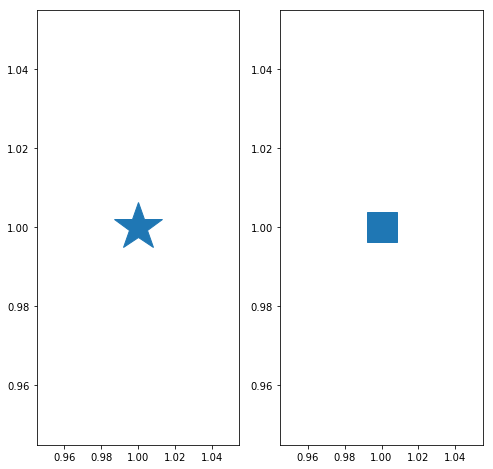
\includegraphics[width=0.8\textwidth]{side_by_side_subplot.png}
\end{figure}

\item
Write the command to create the left subplot (the one that would correspond to the plot with a star in our example figure). Save this subplot in a variable called \texttt{ax1}. \newline
\textbf{Hint:} First, you will have to create the left subplot. Calling \texttt{plt.subplot(1,2,1)} before calling \texttt{plt.plot()} would put a plot in the first column of a 2 column layout with one column.

How would you select the first column of a 2 column layout with one row, instead? What will happen if you change 3rd argument of subplot? i.e. plt.subplot(1,2,2).

\item
Write the command to create the right subplot (the one that would correspond to the plot with a square in our example figure).

Save this subplot in a variable called \texttt{ax2}.
\end{itemize}

\subsubsection{Page Visits Over Time}
In the left subplot, we are going to plot the total page visits over the past year as a line.

\begin{itemize}
\item 
First, let’s create the list of x-values, which is \texttt{range(len(months))}. Store this in a variable called \texttt{x\_values}
    
\item
Make sure this happens after the line where you created \texttt{ax1}, but before the line where you’ve created \texttt{ax2}, so that the plot goes in the subplot on the left.
    
\item
Plot the total page visits against these \texttt{x\_values} as a line.

\item
Give the line markers that will help show each month as a distinct value. \\
\textbf{Hint:} Remember that you can change the marker style inside the call to \texttt{plt.plot} by setting \texttt{marker=<style>} (with \texttt{<style>} representing any of the marker types).

\item
Label the x-axis and y-axis with descriptive titles of what they measure. \\
\textbf{Hint:} \texttt{plt.xlabel} and \texttt{plt.ylabel} will be useful for this.

\item
Set the x-axis ticks to be the \texttt{x\_values}.

\item
Label the x-axis tick labels to be the names stored in the \texttt{months} list. \\
\textbf{Hint:} The \texttt{set\_xticklabels} function of \texttt{ax1} will help you do this task.
\end{itemize}{}

\begin{figure}[htb]
\centering
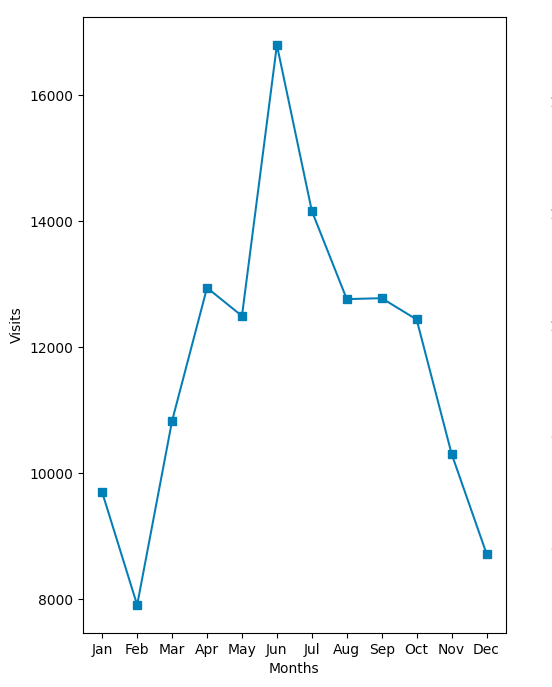
\includegraphics[height=0.8\textwidth]{visits_per_month.png}
\caption{Your left subplot should look like this figure.}\label{fig:visits}
\end{figure}

\subsubsection{Plotting Multiple Lemon Species}
In the subplot on the right, we are going to plot three lines on the same set of axes. The x-values for all three lines will correspond to the months, so we can use the list of \texttt{x\_values} we used for the last plot.

\begin{itemize}
\item 
     On one plot, create the three lines:
    \begin{itemize}
        \item 
        number of citron lemons sold vs \texttt{x\_values}
        \item
        number of Lisbon lemons sold vs \texttt{x\_values}
        \item
        number of sweet lemons sold vs \texttt{x\_values}
    \end{itemize}{}

Make sure this happens after the line where you created \texttt{ax2}, so that it goes in the subplot on the right.

\item
Give each line a specific color of your choosing.

\item
Add a legend to differentiate the lines, labeling each lime species.

\item
Set the x-axis ticks to be the \texttt{x\_values}, and the tick labels to be the \texttt{months} list.
\end{itemize}{}

\newpage

\subsubsection{Labeling and Saving}

\begin{itemize}
\item
Add a title to each of the two plots you’ve created, and adjust the margins to make the text you’ve added look better.

\item
Now, save your figure as a \textit{.png} with a descriptive file name.
\end{itemize}{}

\begin{figure}[htb]
\centering
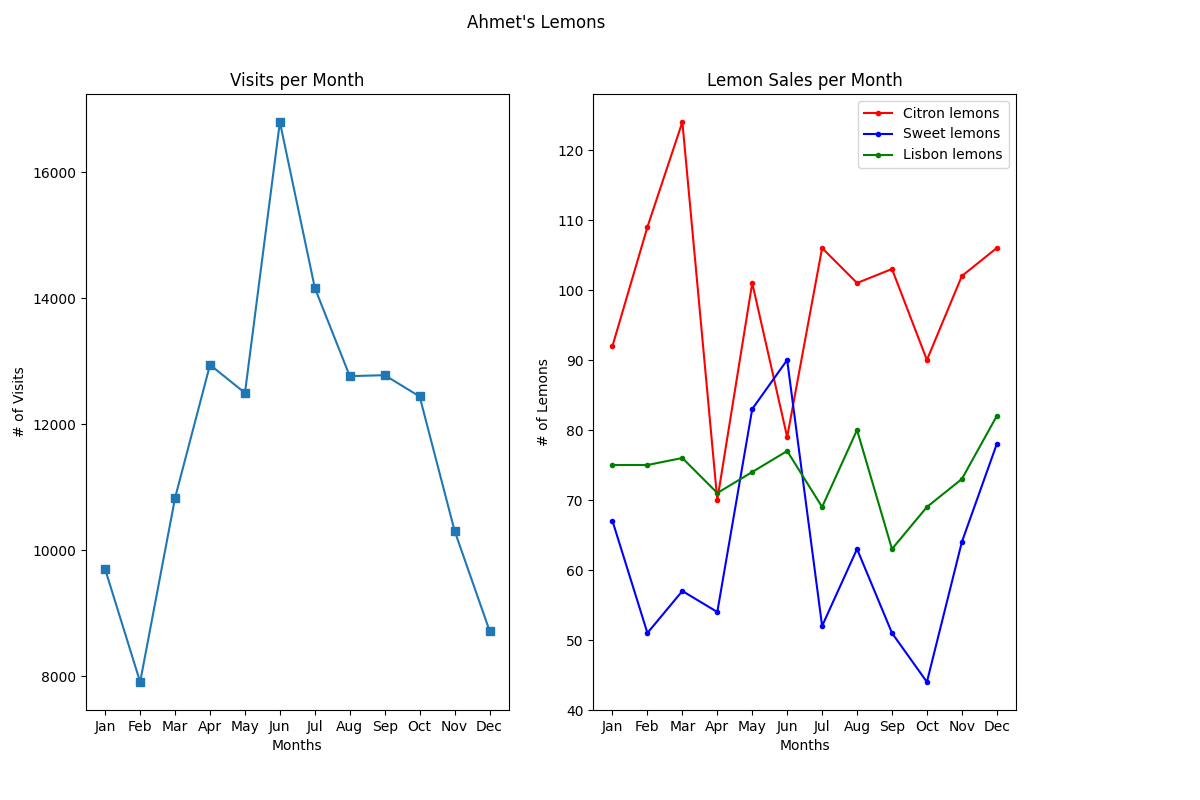
\includegraphics[height=0.8\textwidth]{ahmets_lemons.png}
\caption{Your final plots should look like these figures.}\label{fig:final}
\end{figure}

%Do not change this section.
\subsection{End of Project}
Your project ends here. You may continue to tinker with the code to implement any desired features and discuss them with your section leader. However, \textbf{do not} include any additional features that you implement after this point into your submission. You are just required to submit part 2.2 and 2.4 which are \texttt{cerens\_garden\_center.py} and \texttt{ahmets\_lemons.py}.

\newpage

\section{Resources}
You can find all course and section related material in our \href{https://koltpython.com}{website}. You can download related course slides from \href{https://github.com/koltpython/python-workshops/raw/master/4-Introduction-to-Pandas-and-Matplotlib/pandas_matplotlib_presentation.pdf}{here}. We've also created a \textit{matplotlib} cheatsheet below which can be helpful while implementing the assignment. You can also refer to the official tutorials of \href{https://matplotlib.org/tutorials/index.html}{\textit{matplotlib}} and \href{https://pandas.pydata.org/pandas-docs/stable/reference/index.html}{\textit{pandas}}. 

\subsection{Matplotlib Cheatsheet}
\label{themeMethod}
%This is a list. Lists always begin with this tag. "itemize" describes the list, not begin.
\begin{itemize}

%This is a list item. There is no need to indicate the end for an item as it ends at the next item tag.

\item
\begin{lstlisting}
plt.plot(x_values, y_values)
\end{lstlisting}
Creates a line.  \texttt{x\_values} and  \texttt{y\_values} are lists of
numbers (i.e.,  \texttt{[1, 2, 3, 4]}).
Also accepts the following keyword arguments:

\begin{itemize}
    \item 
    \textbf{\texttt{marker}}: a symbol that will appear at each (x, y)
    point. Options include ‘*’ for a start, ‘o’ for a
    circle, or ‘s’ for a square.
    
    \item 
    \textbf{\texttt{linestyle}}: whether the line is solid (‘-’) or
    dashed (‘--’ or ‘:’) or no line at all (‘’).
   
    \item 
    \textbf{\texttt{linewidth}}: a number representing the thickness
    of the line; default is 1.
    
    \item
    \textbf{\texttt{color}}: the color of the line (can be a HEX code
    or any html color name).
\end{itemize}{}

\item
\begin{lstlisting}
plt.show()
\end{lstlisting}
Displays any previous plot commands.

\item
\begin{lstlisting}
plt.close('all')
\end{lstlisting}
Closes all previous figures.

\item
\begin{lstlisting}
plt.figure(figsize=(width, length))
\end{lstlisting}
Creates a new figure with a specified length and width.
\texttt{width} and \texttt{length} are both numbers in inches.

\item
\begin{lstlisting}
plt.title('My Chart Title')
\end{lstlisting}
A title for a chart.

\item
\begin{lstlisting}
plt.xlabel('My X-Label')
\end{lstlisting}
A label for the x-axis.

\item
\begin{lstlisting}
plt.ylabel('My Y-Label')
\end{lstlisting}
A label for the y-axis


\item
\begin{lstlisting}
plt.subplot(num_rows, num_cols, subplot_index)
\end{lstlisting}
Creates a subplot for a grid with \texttt{num\_rows} rows and
\texttt{num\_cols} columns. The new subplot is at a position
defined by \texttt{subplot\_index}. For instance,
\texttt{plt.subplot(2, 3, 4)} would create a grid with 2
rows and 3 columns and would create a plot in the
second row and the first column (4 “steps” if moving
left to right and top to bottom).

\item
\begin{lstlisting}
ax = plt.subplot()
\end{lstlisting}
Creates and axes object (\texttt{ax}) that can be used for
adjusting the position and labeling of x- and y-axis
tick marks.

\item
\begin{lstlisting}
plt.legend(['label1', 'label2'])
\end{lstlisting}
Creates a legend using the labels given.

\item
\begin{lstlisting}
plt.legend()
\end{lstlisting}
Creates a legend using any \texttt{label} keywords that
were given in \texttt{plt.plot} commands.

\item
\begin{lstlisting}
ax.set_xticks([0, 1, 2, 3, 4])
\end{lstlisting}
Creates tick marks at positions \texttt{[0, 1, 2, 3, 4]}
on the x-axis. \\
Requires that you created an axes object by using
\texttt{ax = plt.subplot()}.

\item
\begin{lstlisting}
ax.set_yticks([0, 1, 2, 3, 4])
\end{lstlisting}
Creates tick marks at positions \texttt{[0, 1, 2, 3, 4]}
on the y-axis. \\
Requires that you created an axes object by using
\texttt{ax = plt.subplot()}.

\item
\begin{lstlisting}
ax.set_xticklabels(['label1', 'label2', 'label3'])
\end{lstlisting}
Modifies the first three labels of the x-axis ticks marks
to be  \texttt{‘label1’, ‘label2’, ‘label3’} \\
Requires that you created an axes object by using
\texttt{ax = plt.subplot().} \\
You’ll probably want to start by specify the positions
of your x-ticks using  \texttt{ax.set\_xticks.}

\item
\begin{lstlisting}
ax.set_yticklabels(['label1', 'label2', 'label3'])
\end{lstlisting}
Modifies the first three labels of the y-axis ticks marks
to be  \texttt{‘label1’, ‘label2’, ‘label3’} \\
Requires that you created an axes object by using
\texttt{ax = plt.subplot().} \\
You’ll probably want to start by specify the positions
of your y-ticks using  \texttt{ax.set\_xticks.}

\item
\begin{lstlisting}
plt.bar(x_values, heights)
\end{lstlisting}
Creates a bar chart with bars at each value of
\texttt{x\_values} using the heights given in \texttt{heights}.
If you’re only creating one bar chart, \texttt{x\_values} can
be equal to \texttt{range(len(heights))}.

\item
\begin{lstlisting}
plt.bar(x_values, heights, bottom=other_heights)
\end{lstlisting}
Creates a second bar chart stacked on top of another
bar chart whose heights are  \texttt{other\_heights}.

\end{itemize}

\end{document}